\subsection{Qualitative Evaluation der Erklärungen}
\label{sec:study_results_qualitativ}

\subsubsection{Ziel der qualitativen Evaluation}

\subsubsection{Methode}

\subsubsection{Ergebnisse}

\begin{figure}[htb!]
    \centering
    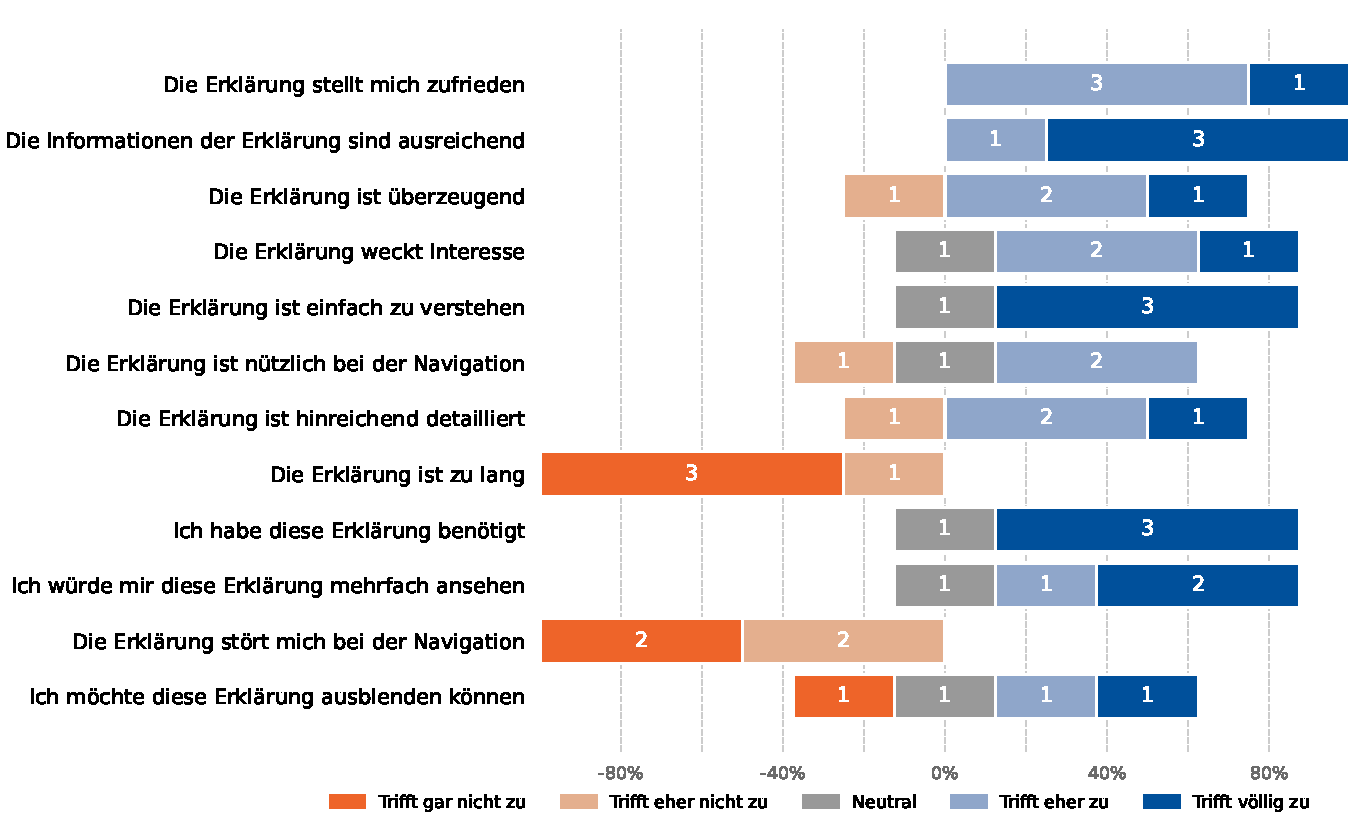
\includegraphics[width=\linewidth]{contents/06_model_evaluation/02_evaluation/res/qualitativeFeedback-01_collaborative_routing.pdf}
    \caption{Qualitative Erklärung 1}
    \label{fig:qualitative_evaluation_explanation1}
\end{figure}

\begin{figure}[htb!]
    \centering
    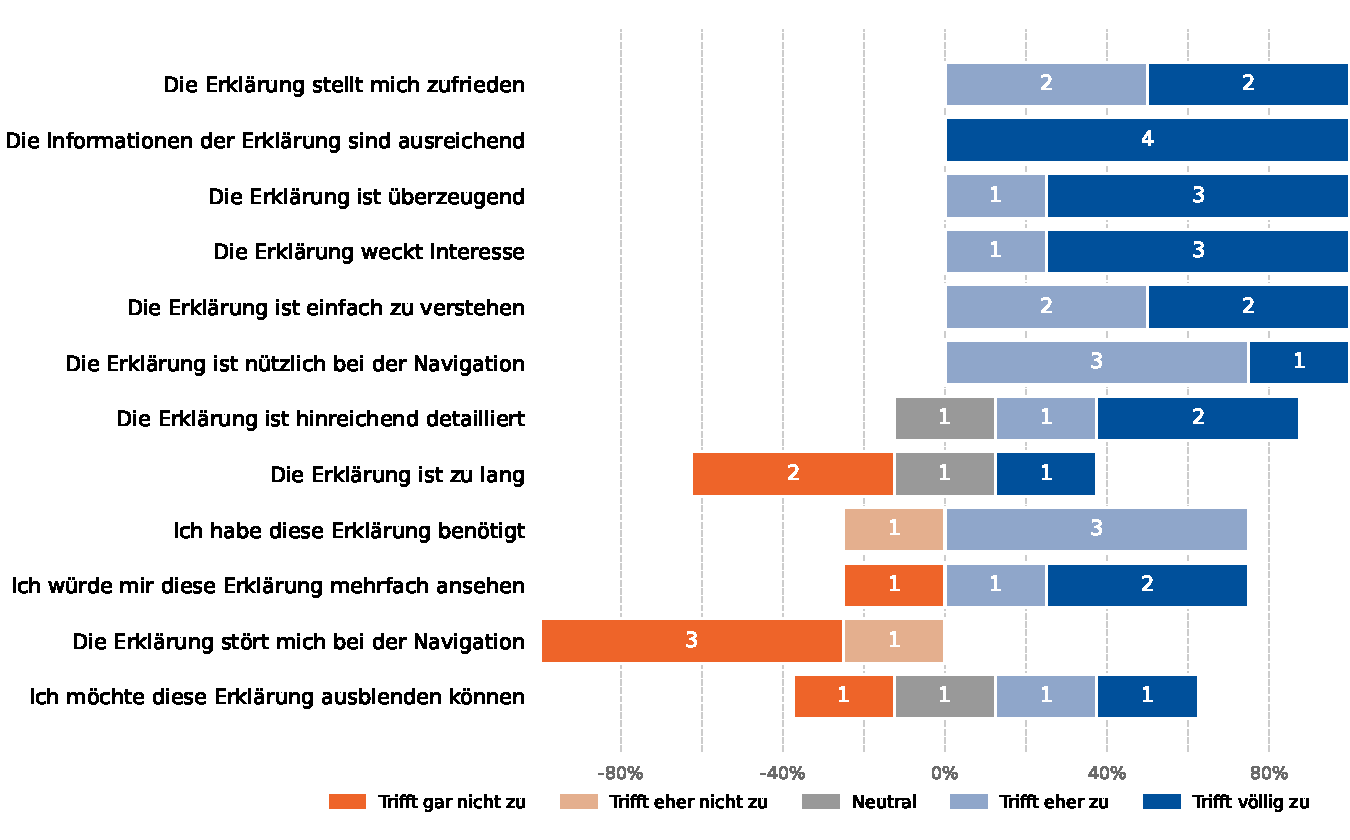
\includegraphics[width=\linewidth]{contents/06_model_evaluation/02_evaluation/res/qualitativeFeedback-02_collaborative_algorithm.pdf}
    \caption{Qualitative Erklärung 2}
    \label{fig:qualitative_evaluation_explanation2}
\end{figure}

\begin{figure}[htb!]
    \centering
    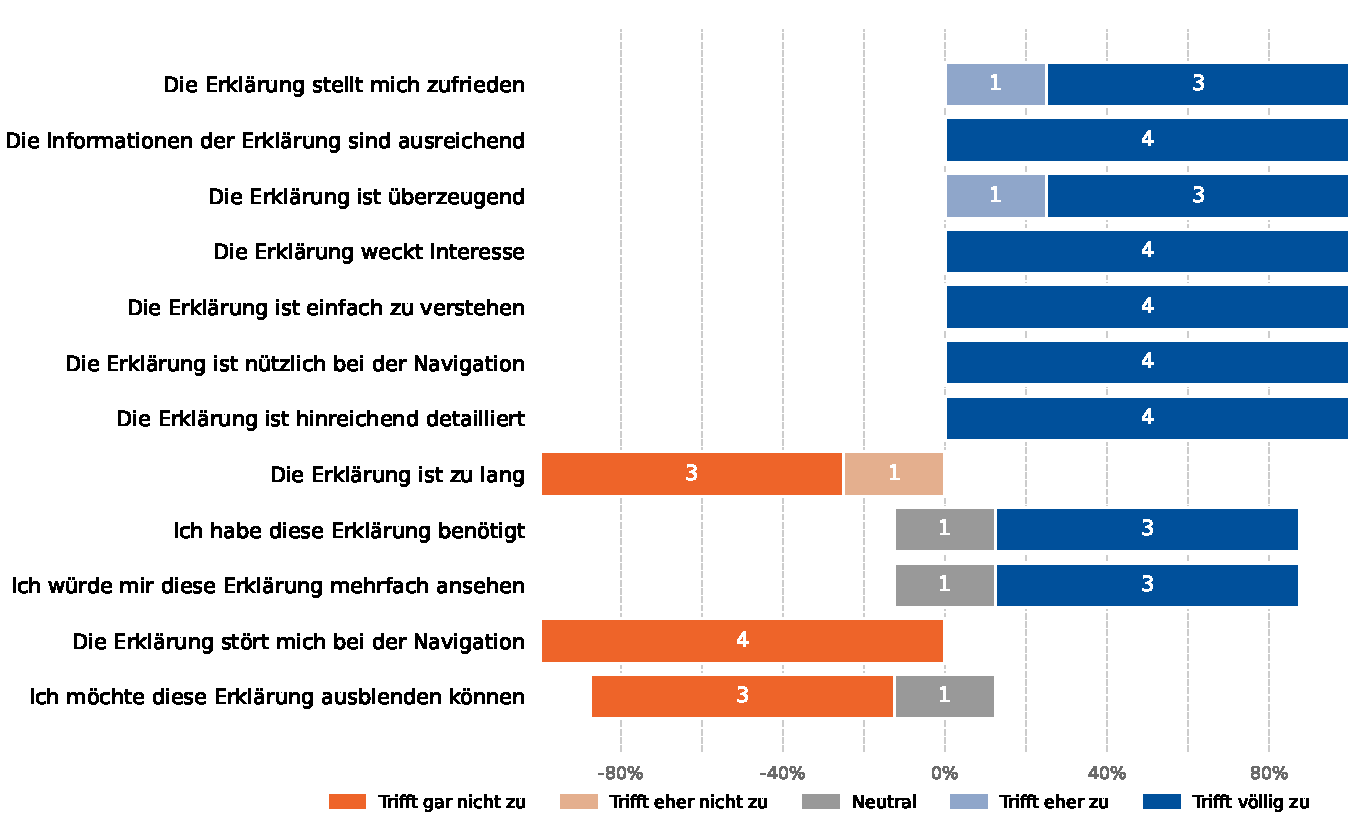
\includegraphics[width=\linewidth]{contents/06_model_evaluation/02_evaluation/res/qualitativeFeedback-03_traffic_volume.pdf}
    \caption{Qualitative Erklärung 3}
    \label{fig:qualitative_evaluation_explanation3}
\end{figure}

\begin{figure}[htb!]
    \centering
    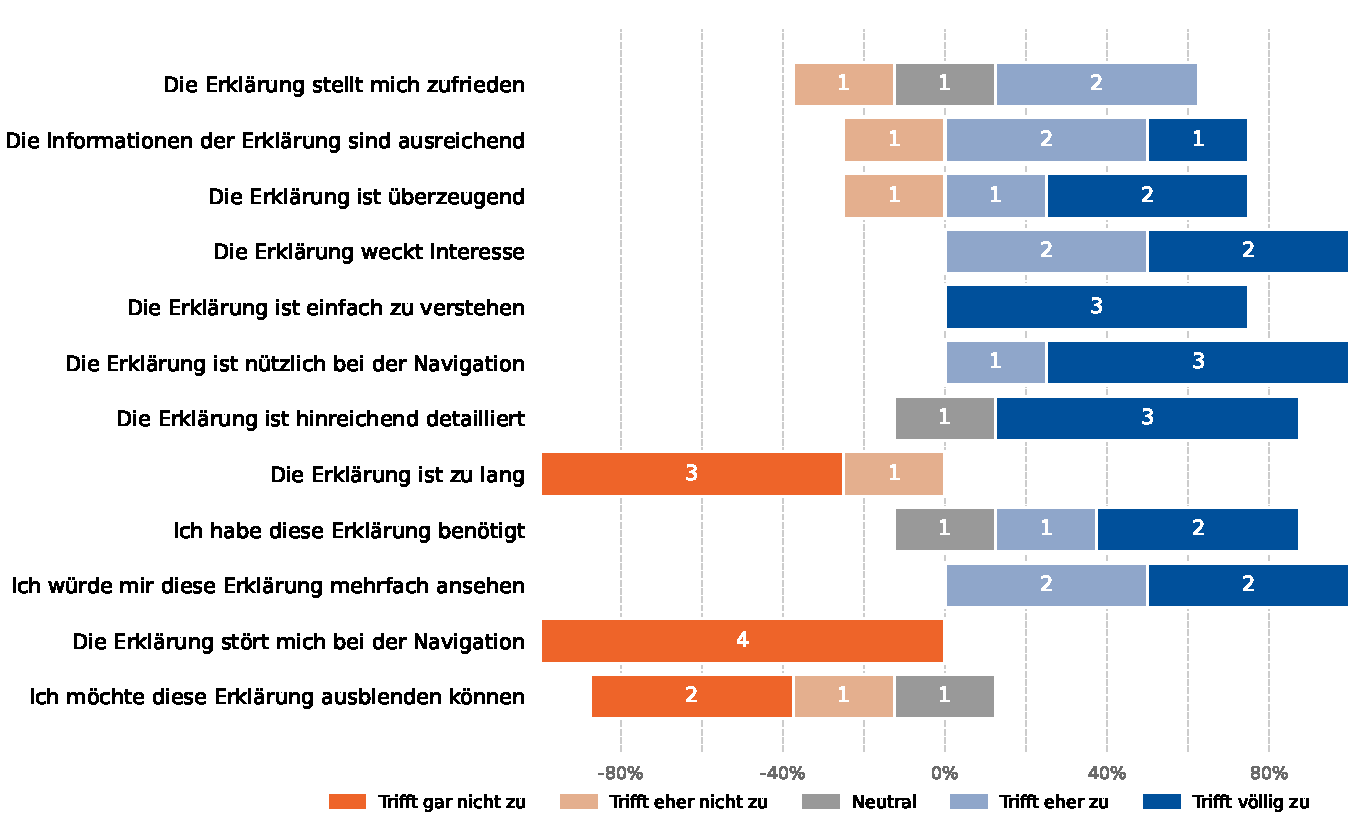
\includegraphics[width=\linewidth]{contents/06_model_evaluation/02_evaluation/res/qualitativeFeedback-04_position_accuracy.pdf}
    \caption{Qualitative Erklärung 4}
    \label{fig:qualitative_evaluation_explanation4}
\end{figure}